% 2009-11-05
\nr

$A_{B}\sim\underbrace{\sum_{\text{alle ZZ}}\efkt{-i\vec{K}\vec{R}}}_{\text{Gitterfaktor}}\underbrace{\sum_{\text{alle Atome}}\efkt{-i\vec{K}\vec{R}}}_{\text{Strukturfaktor}}f_{\alpha}$

\subsection{Strukturfaktor}

$S=\sum_{\text{alle Atome}}f_{\alpha}\efkt{-i\vec{K}\vec{r}_{\alpha}}$
bestimmt Intensit\"at, Ausl\"oschung m\"oglich

\textbf{Beispiel:} bcc Gitter $\vec{r}_{1}=(0,\,0,\,0),\;\vec{r}_{2}=\left(\frac{1}{2},\:\frac{1}{2},\,\frac{1}{2}\right),\quad f_{1}=f_{2}$

aus Gitterfaktor $\vec{K}=\vec{B}=h\vec{b}_{1}+k\vec{b}_{2}+l\vec{b}_{3}\quad h,\, k,\, l\in\mathbb{Z}$

\[
S=f_{1}(\underbrace{\efkt 0}_{1}+\underbrace{\efkt{-i\pi(h+k+l)}}_{\text{gerade =+1, ungerade =-1}}\]



\subsubsection{Atomstrukturfaktor $f_{\alpha}$}

$f_{\alpha}=\int_{\text{Atom }\alpha}\rho_{\alpha}(\vec{r}^{\prime})\efkt{-i\vec{K}\vec{r}^{\prime}}\text{\ensuremath{d^{3}}}\vec{r}^{\prime}$ 

$\rho_{\alpha}$ Streudichte h\"angt von Art der Strahlung ab meist
kugelsymmetrisch

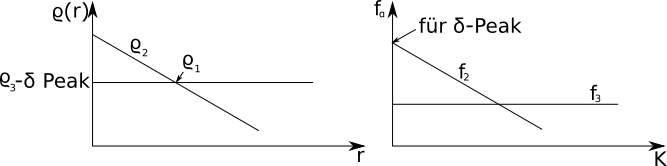
\includegraphics[scale=1]{images/2009-11-05-streugraphen.png}
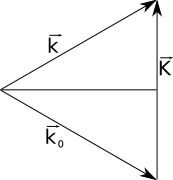
\includegraphics[scale=1]{images/2009-11-05-streu-winkel.png}

bei h\"oheren K d.\,h. bei gr\"o\ss eren Winkeln nimmt Intensit\"at ab.
\begin{labeling}{00.00.0000}
\item [{R\"ontgen:}] \inputencoding{latin1}{$\rho\sim$ Elektronenverteilung,
wie $\rho^{2},\, f_{\alpha}\sim Z$}
\item [{Neutronen:}] $\rho\sim$ Kerne wie $\rho^{3}$
\end{labeling}

\subsubsection{Debye-Wellen-Faktor}

\inputencoding{latin1}%
Temperaturabh\"angigkeit der Streuintensit\"at

$\vec{r}\to\vec{r}(t)=\vec{R}+\vec{r}_{\alpha}+\vec{U}(t)$

$U(t)$ variiert stochastisch d.\,h. thermisch in alle Richtungen
$\langle \vec{U}(t)\rangle =0$

F\"ur Struktur mit 1 Atom auf Gitterpunkt $\vec{r}_{\alpha}=0$

Zus\"atzlich Mittel der Streuamplitude

$\langle A_{B}\rangle =\sum_{\text{alle EZ}}\efkt{-i\vec{K}\vec{R}}\Big(f_{\alpha}\underbrace{\langle \efkt{-i\vec{K}\vec{U}(t)}\rangle }_{T\text{ abh\"{a}ngig}}\Big)$
wobei $\vec{K}=\vec{B}$

$\langle \efkt{-i\vec{K}\vec{U}(t)}\rangle =1-\underbrace{i\langle \vec{K}\vec{U}\rangle }_{=0}-\frac{1}{2}\langle (\vec{U}\vec{K})^{2}\rangle -\ldots$

\begin{wrapfigure}{l}{0.5\columnwidth}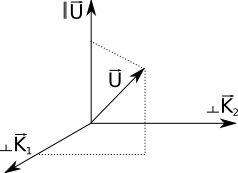
\includegraphics{images/2009-11-05-uparallel.png}\end{wrapfigure}

$\langle (\vec{K}\vec{U})^{2}\rangle =\langle \left(\vec{K}\left(\begin{array}{c}
U_{\parallel K}\\
U_{\perp K_{1}}\\
U_{\perp K_{2}}\end{array}\right)\right)^{2}\rangle =\langle (KU_{\parallel K})^{2}\rangle =K^{2}\langle U_{\parallel K}^{2}\rangle $

$\langle (\vec{U})^{2}\rangle =\langle U_{\parallel}^{2}+U_{\perp K_{1}}^{2}+U_{\perp K_{2}}^{2}\rangle =3\langle U_{\parallel K}^{2}\rangle \Rightarrow\langle U_{\parallel K}^{2}\rangle =\frac{1}{3}\langle U^{2}\rangle $

$\langle \efkt{-i\vec{K}\vec{U}(t)}\rangle =1-\frac{1}{6}K^{2}\langle U^{2}\rangle \approx\efkt{-K^{2}\nicefrac{U^{2}}{6}}$

%
\framebox{\begin{minipage}[t]{1\columnwidth}%
$\Rightarrow\langle A_{b}\rangle \sim\sum_{\text{alle EZ}}\efkt{-i\vec{K}\vec{R}}f_{\alpha}\underbrace{\efkt{-K^{2}\nicefrac{U^{2}}{6}}}_{\text{Debye-Waller-Faktor}}$%
\end{minipage}}


\subsection{Methoden der Strukturanalyse}

\renewcommand{\thesubsubsection}{\alph{subsubsection}) } 


\subsubsection{Verwendete Strahlungsarten f\"ur Beugungsexperimente $\lambda=2a$
Atomabstand}


\paragraph{R\"ontgenstrahlen}

$E=h\nu=\dfrac{hc}{\lambda}$ Streuung an Elektronen, Formfaktor $f\sim Z$,
also $I\sim Z^{2}$, leichte Elemente schwer nachweisbar, benachbarte
Elemente schwer zu unterscheiden, Streuung von Kernen ist vernachl\"assigbar.

Quellen:
\begin{enumerate}
\item R\"ontgenr\"ohre, Bremsstrahlung, hochmagnetisches Elektronen\\
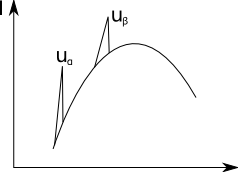
\includegraphics[scale=.75]{images/2009-11-05-bremsstrahlung.png}
\item Synchrotronstrahlung, Elektronen auf Kreisbahn, z.\,B.

\begin{labeling}{00.00.0000}
\item [{ANKA}] Forschungszentrum/Campus Nord
\item [{DESY}] Hamburg
\item [{BESSY}] Berling
\item [{ESRF}] Grenoble
\end{labeling}
\end{enumerate}
hohe Intensit\"at, gepulste Strahl, kleine Divergenz\\
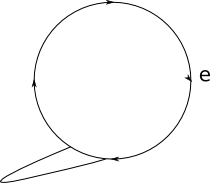
\includegraphics[scale=1]{images/2009-11-05-synchrotron.png}


\paragraph{Neutronen}

$E=\dfrac{p^{2}}{2m}=\dfrac{h^{2}}{2m\lambda^{2}}$ ungeladen, Spin
\inputencoding{latin1}{$\frac{1}{2}$}

Wechselwirkung mit Kernen \"uber starke Wechselwirkung
\begin{itemize}
\item Elektronen in der H\"ulle, die magnetisches Moment tragen geeignet f\"ur
magnetische Strukturen
\end{itemize}

Quellen: Forschungsreaktoren:
\begin{itemize}
\item J\"ulich
\item M\"unchen
\item Grenoble ILL
\item Berlin
\end{itemize}
Wechselwirkung-Querschnitte klein, d.\,h. lange Strahlungszeiten
notwendig

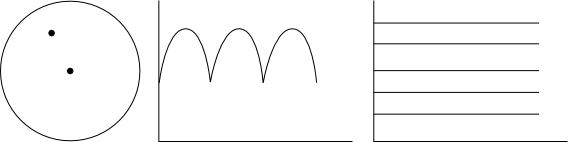
\includegraphics[scale=1]{images/2009-11-05-neutronen.png}


\paragraph{Elektronen}

$E=\dfrac{h^{2}}{2m\lambda^{2}}$ starke Coulomb-Wechselwirkung mit
Elektronen und mit Kernen $\Rightarrow$ nur geringe Eindringtiefe

Oberfl\"achenphysik Low Energy Electron Diffraction: LEED

$E\sim100\,\text{eV}$ Eindringtiefe von wenigen Atomlagen

TEM: d\"unne Schichten herstellen $E\sim\text{keV}$

Vergleich f\"ur $\lambda=1\,\AA$
\begin{labeling}{00.00.0000}
\item [{R\"ontgen}] $\sim\phantom{0}10\,\text{keV}$
\item [{Neutronen}] $\sim100\,\text{meV}$
\item [{Elektronen}] $\sim200\,\text{eV}$
\end{labeling}

\subsubsection{Experimentelle Beugungsverfahren}


\paragraph{Lane-Verfahren: }

kontinuierliches $\lambda$, Einkristall, Ewaldkugel hat ,,dicke
Haut{}``, viele Reflexe gleichzeitig

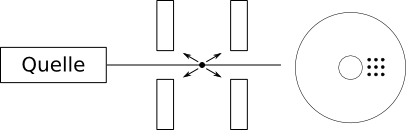
\includegraphics[scale=1]{images/2009-11-05-lane-verfahren.png}
\begin{labeling}{00.00.0000}
\item [{Anwengung:}] Ist die Probe ein Einkristall?\\
Orientierung der Symmetrieachsen
\end{labeling}

\paragraph{Drehristall-Verfahren:}

monochromatische Strahlung, Kristall wird gedreht, Nacheinander treffen
Punkte des reziproken Gitters durch Ewaldkugel

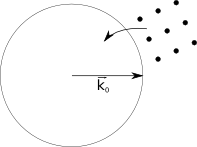
\includegraphics[scale=1]{images/2009-11-05-drehkristall-verfahren.png}


\paragraph{Debye-Scherrer-Verfahren}

monochromatische Strahlung, Pulver oder feink\"orniger Polykristall

\begin{wrapfigure}{o}{0.5\columnwidth}%

\caption[Schnittgebilde: Kreis]%
  {Schnittgebilde: Kreis\\
  Kugel um Ursprung des reziproken Gitters (ende von $\vec{k}_0$) mit Radius des reziproken Gittervektors; \\
  Ewaldkugel mit Radius $\dfrac{2\pi}{\lambda}$}

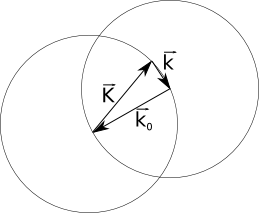
\includegraphics[scale=1]{images/2009-11-05-debye-scherrer-verfahren.png}

\end{wrapfigure}%


Kreis f\"ur alle reziproken Gittervektroren mit $|B|<2|k_{0}|$

Vorteil:
\begin{enumerate}
\item hohe Genauigkeit $\dfrac{\Delta a}{a}\approx10^{-5}$
\item feine Einkristallstruktur
\end{enumerate}
Anwendung: Analyse neuer Verbindungen, komplizierte Kristallstruktur
(Biomolek\"ule) $10^{3}-10^{4}$ Atome pro Einheitszelle


\subsubsection{,,direkte{}`` Abbildung von Strukturen mit atomarer Aufl\"osung}


\paragraph{\uwave{\foreignlanguage{ngerman}{Elektronenmikroskop}} }

de-Broglie-Wellenl\"ange von Elektronen mit $10\,\text{keV}:\;\lambda=0,1\,\AA$
\"ublich $100-400\,\text{keV}$ prinzipiell atomare Aufl\"osung m\"oglich 

Probleme: Linsenfehler $\to$ jetzt gel\"ost


\paragraph{\uwave{Rastertunnel-, Rasterkraftmikroskop} }

images/2009-11-05-rastermikroskope.png
\end{document}
